\documentclass[12pt,letterpaper]{article}
\usepackage[utf8]{inputenc}
\usepackage[T1]{fontenc}
\usepackage{graphicx}
\usepackage{enumitem}
\usepackage{float}
\usepackage{amsmath}
\usepackage{amssymb}
\usepackage{xcolor} 
\usepackage{listings}
\usepackage{hyperref}
%opening
\title{Proyecto de Prolog: Hive}
\author{}
\author{Victor Manuel Cardentey Fundora C411 \and David Guaty Dom\'inguez C412}


\date{}
\lstset{
	columns=fullflexible,
	frame=single,
	breaklines=true,
	postbreak=\mbox{\textcolor{red}{$\hookrightarrow$}\space},
}
\begin{document}

\maketitle
\section*{Estructura del proyecto}
El proyecto consta de 4 m\'odulos:
\begin{enumerate}
	\item app.pl: El m\'odulo encargado de la interacci\'on con el usuario mediante una interfaz gr\'afica realizada en pce.
	\item board.pl: El m\'odulo encargado de modelar la estructura actual de las piezas colocadas. Brinda informaci\'on importante sobre el estado actual del juego.
	\item bugs.pl: EL m\'odulo encargado del manejo de los distintos tipos de insectos. Puede calcular los posibles movimientos de cada insecto.
	\item cpu.pl: El m\'odulo encargado de implementar el jugador no humano.
\end{enumerate}

\section*{board.pl}
\subsection*{Modelado del tablero}
	Aunque el juego no presenta un tablero, el modelado de las posiciones de las piezas sit\'ua las piezas en un grid hexagonal infinito. Para modelar un grid hexagonal se tienen varias opciones, en este proyecto se eligi\'o rotar el eje x del grid de tal forma que cada fila de hex\'agonos est\'a desplaza a la derecha por medio hex\'agono con respecto a la anterior. Por ejemplo, un grid hexagonal de 4x4 se ver\'ia as\'i:
	\begin{figure}[H]
		\centering
		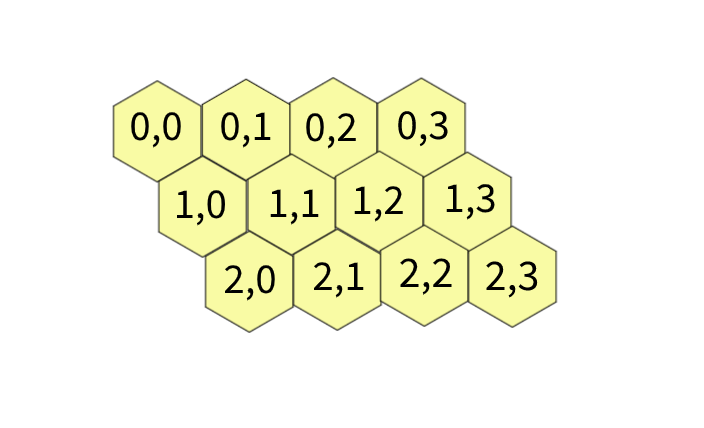
\includegraphics[width=0.7\linewidth]{hexgrid}
		\label{fig:hexgrid}
	\end{figure}

\subsection*{El m\'odulo board}
	Teniendo en cuenta la definici\'on de grid hexagonal anterior, se implement\'o el m\'odulo board para obtener informaci\'on acerca del estado actual del juego.
	
	Para saber si dos casillas son adyacentes se tiene el predicado adyacent(X1, Y1, X2, Y2), que triunfa si el hex\'agono con coordenadas X2,Y2 es adyacente al hex\'agono X1, Y1.
	
	Para llevar el estado del juego, board.pl tiene varios predicados din\'amicos que van cambiando de acuerdo a si se coloca una pieza nueva o si se mueve una pieza. 
	
	Para saber si en la celda con coordenadas X,Y existe un insecto en juego se tiene el predicado bug/5.
	
	bug(C,T,X,Y, S) triunfa si existe un bug de color C( con color se hace referencia a un tipo de jugador), de tipo T(hormiga, reina,etc), que est\'a en la posici\'on X,Y. La variable S se refiere a la posici\'on del insecto dentro de la pila de insectos que se puede formar, por ejemplo un escarabajo que est\'e encima de una reina tendr\'a valor S =1, mientras que la reina tendr\'a valor S=0.
	
	A continuaci\'on se explica como se colocan piezas.
	
	\begin{flushleft}
		\textbf{Celdas fronteras}
	\end{flushleft} 
	 Para colocar un insecto en juego, este tiene que ser adyacente a alg\'un insecto de la colmena, si no se cumple esto se romper\'ia la colmena. Por lo que se tiene la definici\'on de \textbf{celda frontera}. Una celda vac\'ia con coordenadas (X,Y) es \textbf{celda frontera} si es adyacente a una celda no vac\'ia.
	 
	 Para saber si una casilla est\'a vac\'ia se tiene: \textit{empty(X,Y):- $\backslash$+ bug(\_,\_, X, Y, \_) }.
	 
	 \paragraph{} 
	 	\begin{flushleft}
	 	\textbf{Manteniendo almacenadas las celdas fronteras y colocando insectos}
	 \end{flushleft} 
	 Para evitar calcular todas las celdas fronteras cada vez que se vaya a colocar un insecto, se tiene el predicado din\'amico frontier/2, frontier(X,Y) triunfa si la celda con posicion (X,Y) es frontera.
	 
	 Para colocar un insecto en juego se tiene el predicado placeBug(C,T,X,Y): coloca el insecto con color C, de tipo T, en la posici\'on X,Y.
	 
	 Al colocar un nuevo insecto en la celda X,Y que es frontera, se expande la frontera de la colmena, almacenando as\'i las nuevas casillas fronteras. En el placebug se tiene la siguiente l\'inea: \textit{ forall(emptyAdyacent(X,Y,X1,Y1), setFrontier(X1,Y1))}. Tambien se setea un nuevo bug, o sea se a\~nade el predicado bug(C,T,X,Y,0) en la base de datos.
	 
	 Nota: El placeBug hace un poco m\'as, porque tambi\'en sirve para el movimiento de las piezas. El placeBug del m\'odulo escoge la altura de la celda con el predicado getCellHeight(X,Y,H) donde se obtiene en H cuantas piezas hay apiladas en la posici\'on X,Y. El insecto con mayor altura dentro de una celda con altura H es H-1. Luego coloca un bug en la altura H seteando bug(C,T,X,Y,H).
\end{document}